%%%%%%%%%%%%%%%%%%%%%%%%%%%%%%%%%%%%%%%%%%%%%%%%%%%%%%%%%%%%
%%  Class 34, NE 155
%%

\documentclass[xcolor=x11names,compress]{beamer}

\definecolor{CoolBlack}{rgb}{0.0, 0.18, 0.39}
%% General document %%%%%%%%%%%%%%%%%%%%%%%%%%%%%%%%%%
\usepackage{graphicx}
\usepackage{tikz}
\usetikzlibrary{decorations.fractals}
\usepackage{hyperref}
%%%%%%%%%%%%%%%%%%%%%%%%%%%%%%%%%%%%%%%%%%%%%%%%%%%%%%

%% Beamer Layout %%%%%%%%%%%%%%%%%%%%%%%%%%%%%%%%%%
\useoutertheme[subsection=false,shadow]{miniframes}
\useinnertheme{default}
\usefonttheme{serif}
\usepackage{palatino}
\usepackage{tabu}
\usepackage[normalem]{ulem}
% Links
\usepackage{hyperref}
\definecolor{links}{HTML}{003262}
\hypersetup{colorlinks,linkcolor=,urlcolor=links}

% addition of color
\usepackage{xcolor}
\definecolor{CoolBlack}{rgb}{0.0, 0.18, 0.39}
\definecolor{byellow}{rgb}{0.55037, 0.38821, 0.06142}
\definecolor{dgreen}{rgb}{0.,0.6,0.}
\definecolor{RawSienna}{cmyk}{0,0.72,1,0.45}
\definecolor{forestgreen(web)}{rgb}{0.13, 0.55, 0.13}
\definecolor{cardinal}{rgb}{0.77, 0.12, 0.23}

\setbeamerfont{title like}{shape=\scshape}
\setbeamerfont{frametitle}{shape=\scshape}

\setbeamercolor*{lower separation line head}{bg=CoolBlack}
\setbeamercolor*{normal text}{fg=black,bg=white}
\setbeamercolor*{alerted text}{fg=dgreen} % just testing; I think this looks better
\setbeamercolor*{example text}{fg=black}
\setbeamercolor*{structure}{fg=black}

\setbeamercolor*{palette tertiary}{fg=black,bg=black!10}
\setbeamercolor*{palette quaternary}{fg=black,bg=black!10}

% Margins
\usepackage{changepage}

\mode<presentation>
{
  \definecolor{berkeleyblue}{HTML}{003262}
  \definecolor{berkeleygold}{HTML}{FDB515}
  \usetheme{Boadilla}      % or try Darmstadt, Madrid, Warsaw, Boadilla...
  %\usecolortheme{dove} % or try albatross, beaver, crane, ...
  \setbeamercolor{structure}{fg=berkeleyblue,bg=berkeleygold}
  \setbeamercolor{palette primary}{bg=berkeleyblue,fg=white} % changed this
  \setbeamercolor{palette secondary}{fg=berkeleyblue,bg=berkeleygold} % changed this
  \setbeamercolor{palette tertiary}{bg=berkeleyblue,fg=white} % changed this
  \usefonttheme{structurebold}  % or try serif, structurebold, ...
  \useinnertheme{circles}
  \setbeamertemplate{navigation symbols}{}
  \setbeamertemplate{caption}[numbered]
  \usebackgroundtemplate{}
}
%---

\renewcommand{\(}{\begin{columns}}
\renewcommand{\)}{\end{columns}}
\newcommand{\<}[1]{\begin{column}{#1}}
\renewcommand{\>}{\end{column}}

% adding slide numbers
\addtobeamertemplate{navigation symbols}{}{%
    \usebeamerfont{footline}%
    \usebeamercolor[fg]{footline}%
    \hspace{1em}%
    \insertframenumber/\inserttotalframenumber
}

% equation stuff
\newcommand{\Macro}{\ensuremath{\Sigma}}
\newcommand{\Sn}{\ensuremath{S_N} }
\newcommand{\vOmega}{\ensuremath{\hat{\Omega}}}
\usepackage{mathrsfs}
\usepackage[mathcal]{euscript}
\usepackage{amssymb}
\usepackage{amsthm}
\usepackage{epsfig}
\usepackage{amsmath}
%%%%%%%%%%%%%%%%%%%%%%%%%%%%%%%%%%%%%%%%%%%%%%%%%%
% title stuff for footer
\title{NE 155}
\author{R.\ N.\ Slaybaugh \\
(well, Richard Vasques!)}
\date{April 13, 2016}

\begin{document}

%%%%%%%%%%%%%%%%%%%%%%%%%%%%%%%%%%%%%%%%%%%%%%%%%%%%%%
%%%%%%%%%%%%%%%%%%%%%%%%%%%%%%%%%%%%%%%%%%%%%%%%%%%%%%
\begin{frame}
\title{NE 155\\Introduction to Numerical Simulations in Radiation Transport}
\subtitle{Lecture 33: Random Number Generators}
\titlepage
\end{frame}


%%%%%%%%%%%%%%%%%%%%%%%%%%%%%%%%%%%%%%%%%%%%%%%%%%%%%%
%%%%%%%%%%%%%%%%%%%%%%%%%%%%%%%%%%%%%%%%%%%%%%%%%%%%%%
\begin{frame}{Outline}

    \begin{enumerate}
    \item Pseudo-random number sequence vs. \textit{truly} random number sequence
    \item Linear congruential pseudo-random number generators
    \item Define the following:
      \begin{itemize}
      \item Seed
      \item Stride
      \item Period
      \end{itemize}
    \end{enumerate}

\vspace*{1em}
Notes derived from Paul Wilson and K. Ming Leung
\end{frame}

%%%%%%%%%%%%%%%%%%%%%%%%%%%%%%%%%%%%%%%%%%%%%%%%%%%%%%
%%%%%%%%%%%%%%%%%%%%%%%%%%%%%%%%%%%%%%%%%%%%%%%%%%%%%%
\begin{frame}{Random Sequences}
There are two types of random sequences: \textit{truly random} and \textit{pseudo-random}.
\begin{itemize}
\item ``Truly random'' is not a very well-define concept; truly random sequences are undesirable
\begin{itemize}
\item Can be generated by sampling a truly random physical process (e.g. radioactive decay)
\end{itemize}
\item A computer is a deterministic machine and so can never produce truly random sequences
\begin{itemize}
\item It can only represent a finite number of numbers; eventually the numbers have to repeat themselves
\end{itemize}
\item The generators of these ``random'' numbers are known as pseudo-random number generators
\begin{itemize}
\item An algorithm is needed to generate sequences of numbers that appear to be random
\end{itemize}
\end{itemize}

\end{frame}

%%%%%%%%%%%%%%%%%%%%%%%%%%%%%%%%%%%%%%%%%%%%%%%%%%%%%%
%%%%%%%%%%%%%%%%%%%%%%%%%%%%%%%%%%%%%%%%%%%%%%%%%%%%%%
\begin{frame}{Desired Characteristics}

\begin{enumerate}
\item Numbers should be distributed uniformly between 0 and 1 without large ``gaps''
\item Sequence of numbers generated should be as independent from each other as possible
\item Mean or average of the numbers generated should be as close to $1/2$ as possible
\item The variance should be as close to $1/12$ as possible
\item Should have little cyclic variations, i.e. free from the following problems:
\begin{itemize}
\item autocorrelation between numbers
\item numbers successively higher of lower than adjacent numbers
\item several numbers above the mean followed by several numbers below the mean
\end{itemize}
\end{enumerate}

\end{frame}
%%%%%%%%%%%%%%%%%%%%%%%%%%%%%%%%%%%%%%%%%%%%%%%%%%%%%%
%%%%%%%%%%%%%%%%%%%%%%%%%%%%%%%%%%%%%%%%%%%%%%%%%%%%%%
\begin{frame}{Desired Characteristics (continued)}
\begin{enumerate}
\setcounter{enumi}{5}
\item Numbers should have a long cycle
\item Numbers should be replicable, i.e. the same starting condition should yield the same sequence of numbers (for debugging and comparison reasons)
\item The routine that generates these numbers should be extremely fast but should require very little memory
\item The generator should be portable
\end{enumerate}  	
\end{frame}

%%%%%%%%%%%%%%%%%%%%%%%%%%%%%%%%%%%%%%%%%%%%%%%%%%%%%%
%%%%%%%%%%%%%%%%%%%%%%%%%%%%%%%%%%%%%%%%%%%%%%%%%%%%%%
\begin{frame}{Testing Randomness}
\begin{itemize}
\item Not a trivial pursuit
\item NIST defines a set of 15 tests, based in part on different analyses of the bit sequence:
\begin{itemize}
\item Frequency Test: Monobit
\item Frequency Test: Block
\item Runs Test
\item Test for the Longest Runs of Ones in a Block
\item Binary Matrix Rank Test
\item Discrete Fourier Transform (Spectral Test)
\item Non-Overlapping Template Matching Test
\item Overlapping Template Matching Test
\item Maurer's Universal Statistical Test
\item Linear Complexity Test
\item Serial Test
\item Approximate Entropy Test
\item Cumulative Sums Test
\item Random Excursions Test
\item Random Excursions Variant Test
\end{itemize}  	
\end{itemize}  	
\end{frame}

%%%%%%%%%%%%%%%%%%%%%%%%%%%%%%%%%%%%%%%%%%%%%%%%%%%%%%
%%%%%%%%%%%%%%%%%%%%%%%%%%%%%%%%%%%%%%%%%%%%%%%%%%%%%%
\begin{frame}{Visual Comparison}
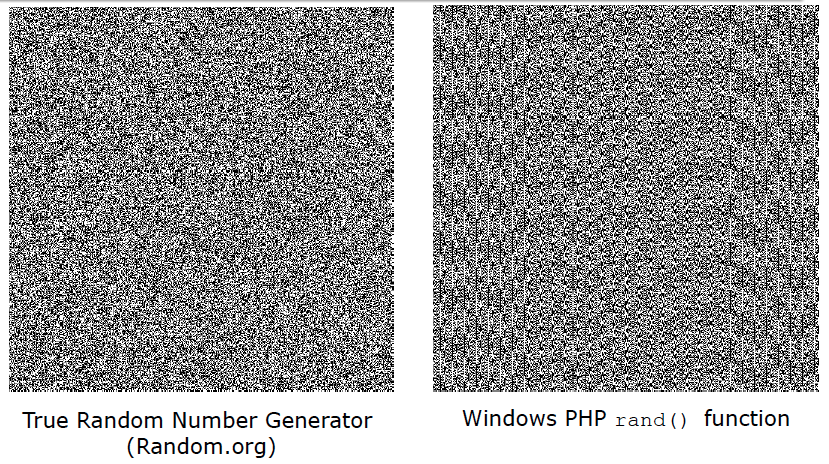
\includegraphics[scale=0.4]{rng1}
\end{frame}

%%%%%%%%%%%%%%%%%%%%%%%%%%%%%%%%%%%%%%%%%%%%%%%%%%%%%%
%%%%%%%%%%%%%%%%%%%%%%%%%%%%%%%%%%%%%%%%%%%%%%%%%%%%%%
\begin{frame}{Linear Congruential PRNG}
\begin{itemize}
\item Simple, fast, robust, well-understood
\item According to Lehmer, 1949:
\begin{align*}
s_{i+1}&=[s_i \times g +c] \text{mod } p\\
r_{i+1}&=\frac{s_{i+1}}{p}
\end{align*}
where  $s_i, g, c, p$ are integers, and $r_i$ are real.
\item Often, $p=2^m$ for integer $m$
\item Selection of $g, c, p$ (or $m$) are important. Moreover:
\begin{itemize}
\item $c=0$: ``multiplicative'' LCPRNG
\item $c\neq 0$: ``mixed" LCPRNG 
\end{itemize}
\end{itemize}  	
\end{frame}

%%%%%%%%%%%%%%%%%%%%%%%%%%%%%%%%%%%%%%%%%%%%%%%%%%%%%%
%%%%%%%%%%%%%%%%%%%%%%%%%%%%%%%%%%%%%%%%%%%%%%%%%%%%%%
\begin{frame}{LCPRNG Parameters}
\begin{itemize}
\item Seed $s_0$
\begin{itemize}
\item The first number in sequence of integers
\item Generally unimportant, but must be known for the sequence to be reproducible
\item Can be changed to force a different result
\end{itemize}
\item Period
\begin{itemize}
\item The number of integers in the sequence before the sequence repeats
\item Generally bad to repeat sequence
\end{itemize}
\end{itemize}  	
\end{frame}

%%%%%%%%%%%%%%%%%%%%%%%%%%%%%%%%%%%%%%%%%%%%%%%%%%%%%%
%%%%%%%%%%%%%%%%%%%%%%%%%%%%%%%%%%%%%%%%%%%%%%%%%%%%%%
\begin{frame}{Typical Parameters}
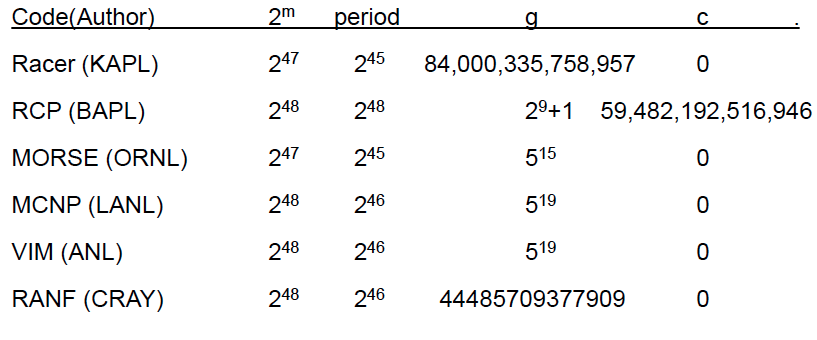
\includegraphics[scale=0.4]{rng2}

Note: $2^{45}$ random numbers can be generated in a few hours
\end{frame}

%%%%%%%%%%%%%%%%%%%%%%%%%%%%%%%%%%%%%%%%%%%%%%%%%%%%%%
%%%%%%%%%%%%%%%%%%%%%%%%%%%%%%%%%%%%%%%%%%%%%%%%%%%%%%
\begin{frame}{General Properties of LCPRNG}
\begin{itemize}
\item The scheme is very simple, reasonably fast, and requires little memory
\item Uniform deviates generated do not continuously fill up the line segment from 0 to 1. They are discrete and can only assume values from the set $0, 1/p, 2/p,...,(p-1)/p$. The smallest possible gap size is $1/p$
\item One can generate at most $p$ distinct numbers before repeating the same sequence of numbers, i.e. the maximum possible cycle length is $p$
\item The modulus operation with $p$ can be conducted efficiently if $p$ is an integer power of $2$ by saving only the rightmost digits. For example if $p = 2m$, then we save only the $m$ rightmost digits
\end{itemize}  	
\end{frame}

%%%%%%%%%%%%%%%%%%%%%%%%%%%%%%%%%%%%%%%%%%%%%%%%%%%%%%
%%%%%%%%%%%%%%%%%%%%%%%%%%%%%%%%%%%%%%%%%%%%%%%%%%%%%%
\begin{frame}{Using PRN sequences in MC Transport}
\begin{itemize}
\item Stride
\begin{itemize}
\item The first random number for history $i$ and history $i+1$ are separated by the stride
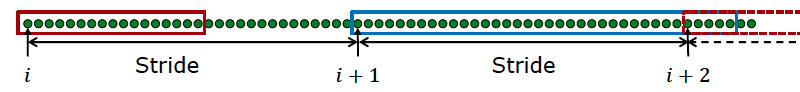
\includegraphics[scale=0.35]{rng3}
\item Most PRNGs have formula to efficiently skip ahead
\begin{itemize}
\item Useful in parallel implementations to spread histories over different processors
\end{itemize}
\item Most histories use only a fraction of the stride
\item Some may exceed the stride
\begin{itemize}
\item Usually OK since numbers will be used to sample very different physical processes
\end{itemize}
\end{itemize}  	
\item Summary
\begin{itemize}
\item The linear congruential pseudo-random number generator is useful for MC sampling
\item The seed, period and stride are interesting to characterize the quality of the PRNG
\end{itemize}
\end{itemize}  	
\end{frame}

%%%%%%%%%%%%%%%%%%%%%%%%%%%%%%%%%%%%%%%%%%%%%%%%%%%%%%
%%%%%%%%%%%%%%%%%%%%%%%%%%%%%%%%%%%%%%%%%%%%%%%%%%%%%%
\begin{frame}{Toy Model}
Consider the LCPRNG having parameters: $c = 0$, $g = 13$, and $p = 2^6 = 64$. \begin{itemize}
\item Using $s_0=1$ as seed:
\begin{itemize}
\item The following sequence of 16 pseudo-random integers is generated: 1, 13, 41, 21, 17, 29, 57, 37, 33, 45, 9, 53, 49, 61, 25, 5
\item After that the sequence repeats itself (the cycle length is 16)
\item Starting with 1, every 4th integer appears in the sequence (the
gap size is $4/64$ = $1/16$ = $0.0625$)
\end{itemize}
\item Using $s_0=2$:
\begin{itemize}
\item The cycle length is 8
\item The gap size is $8/64$ = 0.125
\end{itemize}
\item etc ...
\end{itemize}
\end{frame}

%%%%%%%%%%%%%%%%%%%%%%%%%%%%%%%%%%%%%%%%%%%%%%%%%%%%%%
%%%%%%%%%%%%%%%%%%%%%%%%%%%%%%%%%%%%%%%%%%%%%%%%%%%%%%
\begin{frame}{A Simple Example of MC Simulation}
Consider a circle of radius $r$ inside a square square of side $2r$:
\begin{columns}
	\column{0.30\linewidth}
	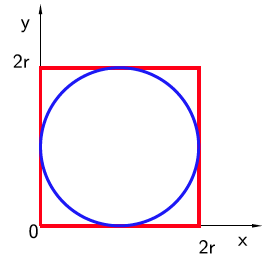
\includegraphics[scale=0.4]{rng4}
	\column{0.65\linewidth}
	\begin{itemize}
	\item Choose $N$ random points in the Square
	\item Let $N'$ be the number of points in the square that are inside the circle
	\item The ratio $N'/N$ must be proportional to [Area Circle]/[Area Square] 
	\end{itemize}
	\end{columns}
	
Therefore:
\[
\frac{N'}{N}\approx\frac{\pi r^2}{4r^2}=\frac{\pi}{4}
\]
and so
\[
\pi \approx 4\frac{N'}{N}.
\]
This suggests a way of computing the value of $\pi$ with the help of a PRNG. 
\end{frame}
%%%%%%%%%%%%%%%%%%%%%%%%%%%%%%%%%%%%%%%%%%%%%%%%%%%%%%
%%%%%%%%%%%%%%%%%%%%%%%%%%%%%%%%%%%%%%%%%%%%%%%%%%%%%%
\begin{frame}{Estimating $\pi$}
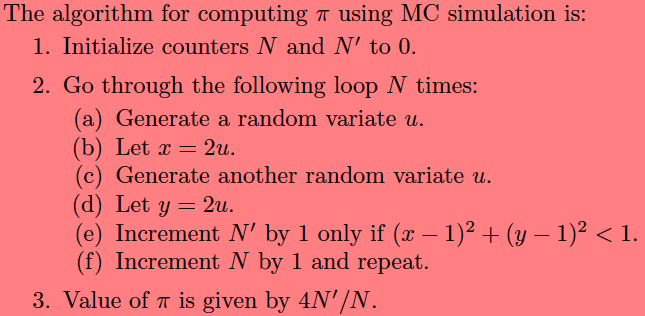
\includegraphics[scale=0.5]{rng5}
\end{frame}

\begin{frame}{Other PRNGs}
\begin{itemize}
\item Middle-square method
\begin{itemize}
\item $s_{k+1}=$ middle digits of $s_k^2$
\end{itemize}
\item Quadratic-congruential
\begin{itemize}
\item $s_{k+1}=[as_k^2+bs_k+c]$mod $p$
\end{itemize}
\item Modified middle-square
\begin{itemize}
\item $s_{k+1}=[s_k(s_k+1)]$mod $p$
\end{itemize}
\item Generalized Additive
\begin{itemize}
\item $s_{k}=[a_1s_{k-1}+a_2s_{k-2}+...+a_is_{k-i}]$mod $p$
\end{itemize}
\end{itemize}  	
\end{frame}

\end{document}